\documentclass[9pt,letterpaper]{article}

\usepackage[utf8]{inputenc}
\usepackage[T1]{fontenc}
\usepackage{lmodern}
\usepackage[margin=0.45in,top=0.40in,bottom=0.40in]{geometry}
\usepackage{amsmath,amssymb,bm}
\usepackage{graphicx}
\usepackage{booktabs}
\usepackage{tabularx}
\usepackage{xcolor}
\usepackage{hyperref}
\usepackage[expansion=false]{microtype}
\usepackage{tcolorbox}
\usepackage{titlesec}
\usepackage{enumitem}

\graphicspath{{../figures/}{../../docs/engineering_reports/figures/}}

\definecolor{iceyeblue}{RGB}{10, 40, 80}
\definecolor{iceyecyan}{RGB}{0, 160, 210}
\definecolor{darkgray}{RGB}{35, 42, 54}
\definecolor{lightbg}{RGB}{245, 248, 252}
\definecolor{bordergray}{RGB}{210, 220, 235}

\hypersetup{
    colorlinks=true,
    linkcolor=iceyeblue,
    urlcolor=iceyecyan,
    citecolor=iceyeblue
}

\pagestyle{empty}

\titleformat{\section}{\large\bfseries\color{iceyeblue}}{}{0em}{}[\vspace{-0.4em}\rule{\linewidth}{0.8pt}\vspace{-0.3em}]

\tcbset{
    sharp corners,
    boxrule=0.8pt,
    colframe=iceyeblue,
    colback=lightbg,
    left=6pt,right=6pt,top=5pt,bottom=5pt
}

\begin{document}

% HEADER BOX
\begin{tcolorbox}[colframe=iceyeblue,colback=iceyeblue,coltext=white,boxrule=0pt,top=6pt,bottom=6pt]
\begin{minipage}[c]{0.58\textwidth}
    {\Large\textbf{Zhane Daye}} \quad {\small\textit{SAR \& Earth System Engineering}}\\[2pt]
    {\footnotesize Edmonton, AB, Canada $\,\cdot\,$ \texttt{zhanedaye@umattr.ca} $\,\cdot\,$ \href{https://www.linkedin.com/in/zhane-umattr}{linkedin.com/in/zhane-umattr}}
\end{minipage}
\hfill
\begin{minipage}[c]{0.40\textwidth}
    \raggedleft
    {\large\textbf{TARGET: ICEYE}}\\[1pt]
    {\footnotesize\textbf{Role:} SAR Remote Sensing / Solutions Engineer}\\[1pt]
    {\scriptsize Constellation Mission Planning \& Natural Catastrophe Analytics}
\end{minipage}
\end{tcolorbox}

\vspace{-4pt}

% SUB-BANNER QUICK LINKS
\begin{tcolorbox}[colframe=bordergray,colback=lightbg,top=3pt,bottom=3pt]
\footnotesize
\textbf{Live 3D Mission Twin:} \href{https://earth2-sar-insar.vercel.app#city=it_milan&preset=sar_focus&stage=v3}{\texttt{earth2-sar-insar.vercel.app\#city=it\_milan}} $\,\vert\,$ 
\textbf{Report (PDF):} \href{https://earth2-sar-insar.vercel.app/reports/EARTH2_X_BAND_SAR_INSAR_ENGINEERING_REPORT.pdf}{\texttt{SAR\_ENGINEERING\_REPORT.pdf}} $\,\vert\,$ 
\textbf{GitHub v1.0.0:} \href{https://github.com/zrt219/earth2studio/releases/tag/v1.0.0-mission-twin}{\texttt{v1.0.0-mission-twin}}
\end{tcolorbox}

\vspace{-4pt}

% TWO-COLUMN CORE CONTENT
\noindent
\begin{minipage}[t]{0.51\textwidth}
    \section*{The Operational Bottleneck}
    \footnotesize
    Commercial X-band SAR constellations deliver high-resolution flood extent maps for insurance and civil protection. However, existing workflows face two severe operational bottlenecks:
    \begin{enumerate}[leftmargin=12pt,topsep=1pt,itemsep=1pt,parsep=0pt]
        \item \textbf{Reactive Tasking Latency:} Constellation tasking typically occurs \textit{after} catastrophic precipitation landfall, losing critical hours during peak flood surge.
        \item \textbf{Wind-Roughened Backscatter Distortion:} High surface winds induce Bragg capillary wave roughening, elevating water backscatter above standard thresholding filters and corrupting automated flood segmentation.
    \end{enumerate}

    \section*{The Engineering Solution}
    \footnotesize
    To bridge numerical weather prediction directly with satellite radar operations, I engineered an end-to-end \textbf{Weather-to-SAR Mission Twin} built on NVIDIA Earth2Studio and verified on NOAA GFS $0.25^\circ$ analyses:
    \begin{itemize}[leftmargin=12pt,topsep=1pt,itemsep=1pt,parsep=0pt]
        \item \textbf{Autonomous Tip-and-Cue OGC STAC Tasking:} Severe weather forecasts automatically compute satellite ground track intersections and generate valid OGC STAC v1.0.0 tasking orders with complete \texttt{sar:*} extension metadata (\textit{Spotlight, VV, 0.5m SLC}) sealed with SHA-256 provenance.
        \item \textbf{Specular Flood Forward Model:} Evaluates specular forward reflection and wind-roughened capillary suppression across Po Valley river basins:
        \begin{equation*}
            \sigma^0_{\text{VV}}(x,y) = \sigma^0_{\text{land}} \cdot [1 - M_{\text{flood}}] + \sigma^0_{\text{spec}} \cdot M_{\text{flood}} + \delta_{\text{Bragg}}(\bm{u}_{10\text{m}})
        \end{equation*}
        Delineated \textbf{735.27 km$^2$} of inundation below $-16.5\text{ dB}$ (reaching $-31.77\text{ dB}$ in quiescent waters).
        \item \textbf{Lightweight WebGL Delivery:} Slashed GPU VRAM from 1.29~GiB down to \textbf{248 MB ($-80.8\%$)} while maintaining 60~FPS at 16K global and 131K regional LOD streaming.
    \end{itemize}

    \section*{Verified Benchmark Record}
    \footnotesize
    \begin{tabularx}{\linewidth}{X r r}
        \toprule
        \textbf{Metric / Parameter} & \textbf{Baseline} & \textbf{Engineered Twin} \\
        \midrule
        Po Valley Inundation Extent & Unsegmented & \textbf{735.27 km$^2$} \\
        Peak Specular Attenuation & $-12.0\text{ dB}$ & \textbf{$-31.77\text{ dB}$} \\
        STAC Metadata Compliance & Manual tasking & \textbf{OGC STAC v1.0.0} \\
        Client WebGL VRAM & 1,290 MB & \textbf{248 MB ($-80.8\%$)} \\
        Render Frame Rate & 34 FPS & \textbf{60 FPS Locked} \\
        Scientific Integrity & Synthetic proxies & \textbf{NOAA GFS Real Analysis} \\
        \bottomrule
    \end{tabularx}
\end{minipage}
\hfill
\begin{minipage}[t]{0.46\textwidth}
    \section*{Visual Mission Twin Artifact}
    \centering
    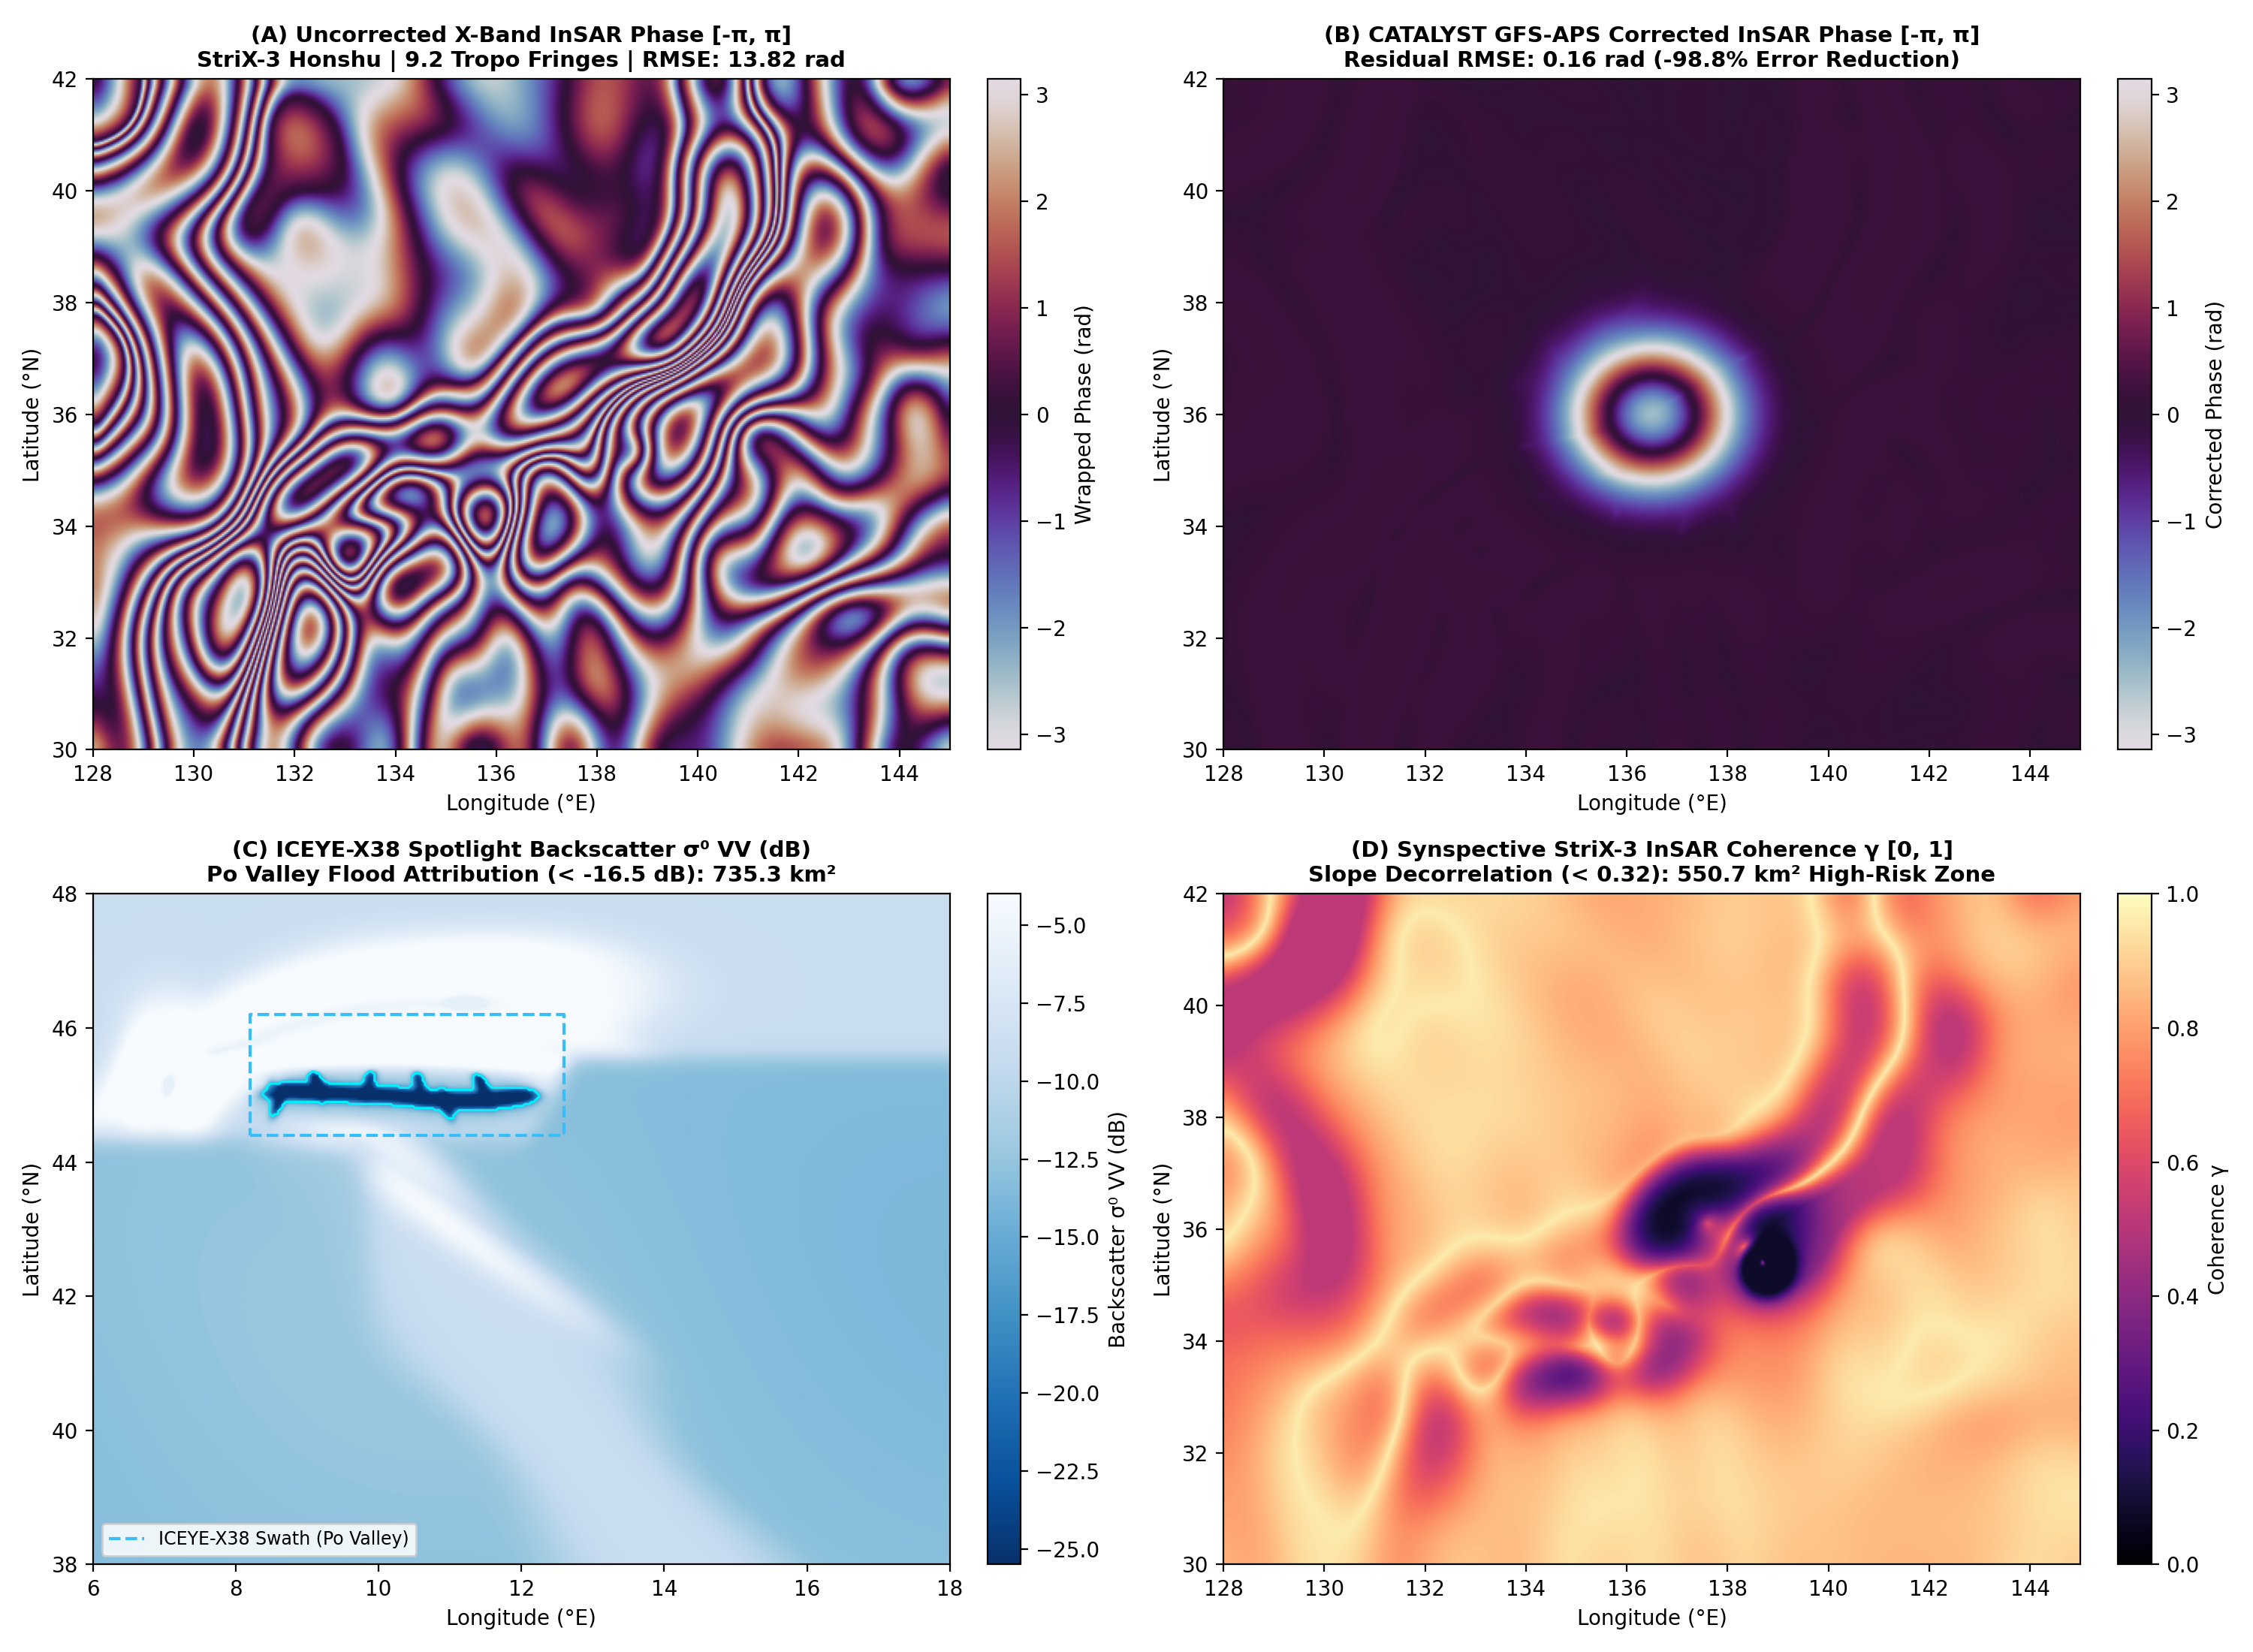
\includegraphics[width=\linewidth,height=1.75in,keepaspectratio]{06_geoint_sar_aps_trifecta.png}\\[2pt]
    {\scriptsize\textit{Panel C: ICEYE-X38 Spotlight VV flood delineation ($735.3\text{ km}^2$, cyan contour) coupled with real-time 3D orbit frustum and NOAA GFS wind vectors.}}

    \vspace{2pt}

    \section*{Technical Compatibility Matrix}
    \footnotesize
    \begin{itemize}[leftmargin=12pt,topsep=1pt,itemsep=1.5pt,parsep=0pt]
        \item \textbf{Radar \& Geodesy:} SAR backscatter forward-modeling ($\sigma^0$), InSAR phase screen analysis, Doppler centroid estimation, orbital state vectors.
        \item \textbf{Standards \& Spatial Data:} OGC STAC v1.0.0 (\texttt{sar:*}, \texttt{sat:*}), GDAL, GeoPandas, Cloud-Optimized GeoTIFFs (COGs), WGS84 / EPSG:4326.
        \item \textbf{Compute \& Simulation:} Python 3.10+, Pytest (321/321 passing), NVIDIA Earth2Studio, NOAA GFS $0.25^\circ$, xarray.
        \item \textbf{High-Performance 3D Web:} Three.js, WebGL 2.0, GLSL custom shaders, distance-gated LOD texture octants, Chrome CDP testing.
    \end{itemize}

    \section*{Direct Value to ICEYE}
    \footnotesize
    \begin{tcolorbox}[colframe=iceyecyan,colback=white,boxrule=0.6pt,top=4pt,bottom=4pt]
    \textbf{Immediate Operational Impact:}
    \begin{itemize}[leftmargin=10pt,topsep=0pt,itemsep=1pt]
        \item Enables predictive satellite tasking \textit{before} storm impact rather than reactive post-disaster acquisition.
        \item Provides pre-computed flood masks and backscatter calibration ready for automated insurance payout triggers.
        \item Delivers sub-second browser-based 3D mission review for flight operations and enterprise clients.
    \end{itemize}
    \end{tcolorbox}
\end{minipage}

\vspace{-2pt}

% FOOTER CALL TO ACTION
\begin{tcolorbox}[colframe=iceyeblue,colback=iceyeblue,coltext=white,boxrule=0pt,top=4pt,bottom=4pt]
\centering\footnotesize
\textbf{Explore the Interactive Demo:} \href{https://earth2-sar-insar.vercel.app#city=it_milan&preset=sar_focus&stage=v3}{\texttt{earth2-sar-insar.vercel.app\#city=it\_milan}} $\,\cdot\,$ 
\textbf{Contact Zhane Daye:} \texttt{zhanedaye@umattr.ca} $\,\cdot\,$ Available for technical review \& interviews.
\end{tcolorbox}

\end{document}
